
\chapter{面积}
\label{chap:area}

\section{基本公式}
\label{sec:basic-area-formula}

% \begin{table}[htbp]
%   \centering
%   \renewcommand{\arraystretch}{1.2}
%   % The > directive lets you basically inject the contained code
%   % before each entry in that column.
%   % 
%   % The point of \arraybackslash is to return \\ to its original
%   % meaning because the \centering command alters this and could
%   % possibly give you a noalign error during compilation.
%   % \newcolumntype{C}{ >{\centering\arraybackslash} m{1cm} }
%   % \newcolumntype{D}{ >{\centering\arraybackslash} m{2cm} }
%   % \newcolumntype{E}{ >{\centering\arraybackslash} m{4cm} }
%   % \newcolumntype{F}{ >{\centering\arraybackslash} m{6cm} }

%   % define "struts", as suggested by Claudio Beccari in
%   % a piece in TeX and TUG News, Vol. 2, 1993.
%   % \newcommand\Tstrut{\rule{0pt}{2.6ex}}         % = `top' strut
%   % \newcommand\Bstrut{\rule[-0.9ex]{0pt}{0pt}}   % = `bottom' strut
  
%   \begin{tabular}{cccl}
%     \hline
%     序号&图形 & 示例 & 公式\\
%     \hline\\[2pt]
%     1 & 三角形 & \tikz{\draw(2,2)--(0,0)--(3,0)--(2,2)--(2,0)
%                             (1.8,0)--(1.8,.2)--(2,.2);
%                  \draw[|<->|](0,-.3)--(3,-.3)node[midway,fill=white]{$a$};
%                  \draw[|<->|](3.5, 0)--(3.5, 2)node[midway,fill=white]{$h$};
%                  } & $S=\frac12 ah$\\
%     2 & 矩阵 & \tikz{
%                \draw(0,0)rectangle(3,2);
%                \draw[|<->|](0,-.3)--(3,-.3)node[midway,fill=white]{$a$};
%                \draw[|<->|](3.5,0)--(3.5,2)node[midway,fill=white]{$b$};
%                } & $S=ab$\\
%     \hline
%   \end{tabular}
%   \caption{基本面积公式}
%   \label{tab:basic-area-formula}
% \end{table}

一些基本图形的面积公式列表如下:
\begin{center}
\begin{tikzpicture}
  \begin{scope}[shift={(0,0)}]
    \draw(2,2)--(0,0)--(3,0)--(2,2)--(2,0)
    (1.8,0)--(1.8,.2)--(2,.2);
    \draw[|<->|](0,-.3)--(3,-.3)node[midway,fill=white]{$a$};
    \draw[|<->|](3.5, 0)--(3.5, 2)node[midway,fill=white]{$h$};
    \node[right]at (4,1){$S=\dfrac12 ah$};
  \end{scope}

  \begin{scope}[shift={(8,0)}]
    \draw(0,0)rectangle(3,2);
    \draw[|<->|](0,-.3)--(3,-.3)node[midway,fill=white]{$a$};
    \draw[|<->|](3.5,0)--(3.5,2)node[midway,fill=white]{$b$};
    \node[right]at (4,1){$S=ab$};
  \end{scope}

  \begin{scope}[shift={(0,-4)}]
    \draw[|<->|](1,2.3)--(2.5,2.3)node[midway,fill=white]{$b$};
    \draw[|<->|](0,-.3)--(3,-.3)node[midway,fill=white]{$a$};
    \draw[|<->|](3.5,0)--(3.5,2)node[midway,fill=white]{$h$};
    \draw(0,0)--(3,0)--(2.5,2)--(1,2)--cycle;
    \node[right]at (4,1){$S=\dfrac12 (a+b)h$};
  \end{scope}

  \begin{scope}[shift={(8,-4)}]
    \draw(1.5,1)circle(1.5);
    \draw[->](1.5,1)--(3,1)node[midway,above]{$r$};
    \node[right]at(4,1){$S=\pi r^2$};
  \end{scope}

  \begin{scope}[shift={(0,-8)}]
    \draw(0,1)node(O){}--(3,1)node(A){} arc(0:30:3) node(B){}--cycle;
    \draw[|<->|](0,.6)--(3,.6)node[midway,below]{$r$};
    \draw pic["$\theta$",<->,draw=orange,angle eccentricity=1.6,angle radius=.6cm]{angle=A--O--B};
    \node[right]at(4,1.5){$S=\dfrac12 \theta r^2$};
  \end{scope}
\end{tikzpicture}
\end{center}

\begin{example}
  已知正方形边长,求阴影面积。

  \centering
  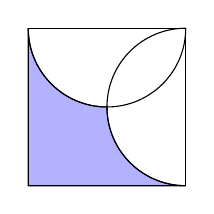
\begin{tikzpicture}[scale=2.0]
    \draw[fill=blue!30](0,0)--(1,0)arc(-90:-180:.5)arc(-90:-180:.5)--cycle;
    \draw(0,0)--(1,0)--(1,1)--(0,1)--cycle;
    \draw(1,0)arc(-90:-270:.5) (1,1)arc(0:-180:.5);
  \end{tikzpicture}
\end{example}

\hints 作辅助线,分别求各部分面积。

\begin{center}
  \begin{tikzpicture}[scale=2.0]
    % \draw[fill=blue!30](0,0)--(1,0)arc(-90:-180:.5)arc(-90:-180:.5)--cycle;
    \draw(0,0)--(1,0)--(1,1)--(0,1)--cycle;
    \draw(1,0)arc(-90:-270:.5) (1,1)arc(0:-180:.5);
    \draw[dashed,pattern=north east lines,pattern color=blue!30](.5,.5)rectangle(1,1);
  \end{tikzpicture}
\end{center}

\begin{example}
  求阴影面积

  \centering
  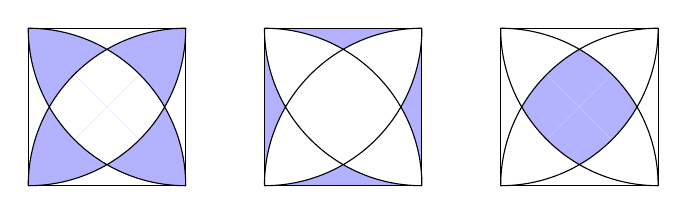
\begin{tikzpicture}[scale=1.0]
    \begin{scope}[shift={(0,0)}]
      \draw(0,0)rectangle(2,2);
      \draw[fill=blue!30,even odd rule]
           ([shift=(0:2)]0,0)arc(0:90:2)
           ([shift=(90:2)]2,0)arc(90:180:2)
           ([shift=(180:2)]2,2)arc(180:270:2)
           ([shift=(270:2)]0,2)arc(270:360:2);
    \end{scope}

    \begin{scope}[shift={(3,0)}]
      \fill[color=blue!30] (0,0)--(2,0) arc(-90:-120:2) arc(-60:-90:2);
      \fill[color=blue!30] (2,0)--(2,2) arc(0:-30:2) arc(30:0:2);
      \fill[color=blue!30] (2,2)--(0,2) arc(90:60:2) arc(120:90:2);
      \fill[color=blue!30] (0,2)--(0,0) arc(180:150:2) arc(210:180:2);
      \draw(0,0)rectangle(2,2);
      \draw([shift=(0:2)]0,0)arc(0:90:2)
           ([shift=(90:2)]2,0)arc(90:180:2)
           ([shift=(180:2)]2,2)arc(180:270:2)
           ([shift=(270:2)]0,2)arc(270:360:2);
    \end{scope}

    \begin{scope}[shift={(6,0)}]
      \fill[color=blue!30]
           ([shift=(0:2)]0,0)arc(0:90:2)
           ([shift=(90:2)]2,0)arc(90:180:2)
           ([shift=(180:2)]2,2)arc(180:270:2)
           ([shift=(270:2)]0,2)arc(270:360:2);
      \fill[color=white,even odd rule]
           ([shift=(0:2)]0,0)arc(0:90:2)
           ([shift=(90:2)]2,0)arc(90:180:2)
           ([shift=(180:2)]2,2)arc(180:270:2)
           ([shift=(270:2)]0,2)arc(270:360:2);
      \draw(0,0)rectangle(2,2);
      \draw([shift=(0:2)]0,0)arc(0:90:2)
           ([shift=(90:2)]2,0)arc(90:180:2)
           ([shift=(180:2)]2,2)arc(180:270:2)
           ([shift=(270:2)]0,2)arc(270:360:2);
    \end{scope}
  \end{tikzpicture}
\end{example}
\begin{proof}[解]
  交点将圆弧平均分成三段,每段对应于$30^\circ$的圆弧。\hints 图中三角形是等边三角形。

  \begin{center}
  \begin{tikzpicture}[scale=1.0]
    \draw(0,0)rectangle(2,2);
    \draw([shift=(0:2)]0,0)arc(0:90:2)
         ([shift=(90:2)]2,0)arc(90:180:2)
         ([shift=(180:2)]2,2)arc(180:270:2)
         ([shift=(270:2)]0,2)arc(270:360:2);
    \coordinate (A) at (60:2);
    \draw[very thick](0,0)--(2,0)--(A)--cycle;
    \fill[pattern=north west lines,pattern color=blue!30](0,0)--(A)arc(60:90:2)--cycle;
    \fill[pattern=north east lines,pattern color=blue!30](2,0)--(2,2)arc(90:120:2)--cycle;
  \end{tikzpicture}
  \end{center}

  可按图中分割方式求解题目第二个图中阴影面积。
\end{proof}

\begin{example}
  由两个圆弧组成的图形称为半月形(lune)。求图中阴影部分半月形的面积。

  \centering
  \begin{tikzpicture}[scale=1.5]
    \coordinate (O) at (0,0);
    \coordinate (A) at (120:1); 
    \coordinate (B) at (60:1);
    \coordinate (C) at ($.5*(A) + .5*(B)$);
    \draw[fill=blue!30](B)arc(0:180:.5);
    \draw[fill=white](1,0)arc(0:180:1);
    \draw[dashed](A)--(B) node[midway,below]{$1$};
    \draw(-1,0)--(1,0) node[midway, below]{$2$};;
  \end{tikzpicture}
\end{example}
\begin{proof}[提示]
  可转换为求弓形面积。

  \begin{center}
    \begin{tikzpicture}[scale=2.0]
      \coordinate (O) at (0,0);
      \coordinate (A) at (120:1);
      \coordinate (B) at (60:1);
      \draw[pattern=north west lines, pattern color=blue!30](A)--(B) arc(60:120:1);
      \draw(A)--(O)--(B);
    \end{tikzpicture}
  \end{center}

  弓形面积可由上图中分割方式求出,即扇形面积减三角形面积。
\end{proof}

\begin{example}
  图中四边形为单位正方形,求阴影面积。

  \centering
  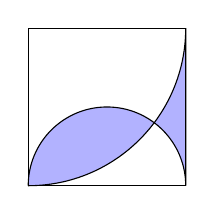
\begin{tikzpicture}[scale=1.0]
    \draw[fill=blue!30,even odd rule](0,0)arc(-90:0:2)--(2,0)arc(0:180:1);
    \draw(2,0)--(0,0)--(0,2)--(2,2);
  \end{tikzpicture}
\end{example}
\begin{proof}[解]
  除了积分,暂时未发现有其它好方法。
  \begin{align*}
    S&=\int_{x=0}^1 \left| \sqrt{0.5^2 - (x-0.5)^2} - \left(1-\sqrt{1-x^2}\right)\right| \dx\qedhere
  \end{align*}
\end{proof}

\begin{example}
  已知三角形面积为$1$,求阴影面积。其中第一个图的线段长度的比例如图所示。后两图,若其中线段长度的比例都已知,则阴影面积又该如何求解?

  \centering
  \begin{tikzpicture}[scale=1.0]
    \begin{scope}[shift={(0,0)}]
      \coordinate (A) at (1.8,2);
      \coordinate (B) at (0,0);
      \coordinate (C) at (3,0);
      \coordinate (D) at ($.6*(C)$);
      \coordinate (E) at ($2/3*(A)+1/3*(C)$);
      \draw(A)--(B)--(C)--cycle (D)--(E);
      \fill[pattern=north west lines,pattern color=blue!30](C)--(D)--(E)--cycle;

      \coordinate (B') at ($(0,-.4) + (B)$);
      \coordinate (C') at ($(0,-.4) + (C)$);
      \coordinate (D') at ($(0,-.4) + (D)$);
      \draw[|<->|](B')--(D') node[midway,below]{$3x$};
      \draw[|<->|](D')--(C') node[midway,below]{$2x$};

      \coordinate (P)  at ($({.4*2/sqrt(5.44)}, {.4*1.2/sqrt(5.44)})$);
      \coordinate (C') at ($(P) + (C)$);
      \coordinate (E') at ($(P) + (E)$);
      \coordinate (A') at ($(P) + (A)$);
      \draw[|<->|](C')--(E') node[pos=.75,above right,sloped]{$2y$};
      \draw[|<->|](E')--(A') node[pos=.75,above right,sloped]{$y$};
    \end{scope}

    \begin{scope}[shift={(4.5,0)}]
      \coordinate (B) at (0,0);
      \coordinate (C) at (3,0);
      \coordinate (A) at (2,2);
      \coordinate (D) at ($.4*(B) + .6*(C)$);
      \coordinate (E) at ($.3*(A) + .7*(C)$);
      \coordinate (F) at ($.5*(A) + .5*(B)$);
      \draw(A)--(B)--(C)--cycle;
      \draw[pattern=north west lines,pattern color=blue!30](D)--(E)--(F)--cycle;
    \end{scope}

    \begin{scope}[shift={(9,0)}]
      \coordinate (B) at (0,0);
      \coordinate (C) at (3,0);
      \coordinate (A) at (2,2);
      \coordinate (D) at ($.4*(B) + .6*(C)$);
      \coordinate (E) at ($.3*(A) + .7*(C)$);
      \coordinate (F) at ($.5*(A) + .5*(B)$);
      \coordinate (G) at ($.8*(B) + .2*(C)$);
      \draw(A)--(B)--(C)--cycle;
      \draw[pattern=north west lines,pattern color=blue!30](D)--(E)--(F)--(G)--cycle;
    \end{scope}

  \end{tikzpicture}
\end{example}
\begin{proof}[解]\mbox{}\\
  \begin{center}
    \begin{tikzpicture}[scale=1.0]
    \begin{scope}[shift={(0,0)}]
      \coordinate (A) at (1.8,2);
      \coordinate (B) at (0,0);
      \coordinate (C) at (3,0);
      \coordinate (D) at ($.6*(C)$);
      \coordinate (E) at ($2/3*(A)+1/3*(C)$);
      \draw(A)--(B)--(C)--cycle (D)--(E);
      \fill[pattern=north west lines,pattern color=blue!30](C)--(D)--(E)--cycle;

      \coordinate (B') at ($(0,-.4) + (B)$);
      \coordinate (C') at ($(0,-.4) + (C)$);
      \coordinate (D') at ($(0,-.4) + (D)$);
      \draw[|<->|](B')--(D') node[midway,below]{$3x$};
      \draw[|<->|](D')--(C') node[midway,below]{$2x$};

      \coordinate (P)  at ($({.4*2/sqrt(5.44)}, {.4*1.2/sqrt(5.44)})$);
      \coordinate (C') at ($(P) + (C)$);
      \coordinate (E') at ($(P) + (E)$);
      \coordinate (A') at ($(P) + (A)$);
      \draw[|<->|](C')--(E') node[pos=.75,above right,sloped]{$2y$};
      \draw[|<->|](E')--(A') node[pos=.75,above right,sloped]{$y$};

      \draw[dashed](A)--(D);
    \end{scope}
  \end{tikzpicture}
\end{center}

  作辅助线,可以容易看出各个三角形之间的面积关系。
\end{proof}

\section{面积法}
\label{sec:area-method}

有时解决问题可以升维或降维。比如在某些情况下求解线段问题时,可以升维成面积问题。反之,有时求解体积问题时可以降维成线段问题。

\begin{example}
  如图,$D$和$E$是$\triangle ABC$两边上一点,$O$是$AE$与$CD$的交点。若$\dfrac{CE}{BE}=\dfrac{u}{v}$,$\dfrac{AD}{BD}=\dfrac{x}{y}$,求$\dfrac{CO}{DO}$。
  \begin{center}
    \begin{tikzpicture}[scale=1.5]
      \coordinate[label=below left:$A$](A) at (0,0);
      \coordinate[label=below right:$B$](B) at (3,0);
      \coordinate[label=above:$C$](C) at (2,2);
      \coordinate[label=below:$D$](D) at ($.6*(A)+.4*(B)$);
      \coordinate[label=right:$E$](E) at ($.5*(B)+.5*(C)$);
      \coordinate[label=above left:$O$](O) at ($2/7*(C)+5/7*(D)$);
      \draw(A)--(D) node[midway,below]{$x$};
      \draw(D)--(B) node[midway,below]{$y$};
      \draw(B)--(E) node[midway,right]{$v$};
      \draw(E)--(C) node[midway,right]{$u$};
      \draw(C)--(A)--(O)--(E) (C)--(D);
      \tkzDrawPoints(A,B,C,D,E,O)
    \end{tikzpicture}
  \end{center}
\end{example}
\begin{proof}[提示]利用面积法。如图,设$\triangle AOD$与$\triangle COE$的面积分别为$M$和$N$。
  \begin{center}
    \begin{tikzpicture}[scale=1.5]
      \begin{scope}
        \coordinate[label=below left:$A$](A) at (0,0);
        \coordinate[label=below right:$B$](B) at (3,0);
        \coordinate[label=above:$C$](C) at (2,2);
        \coordinate[label=below:$D$](D) at ($.6*(A)+.4*(B)$);
        \coordinate[label=right:$E$](E) at ($.5*(B)+.5*(C)$);
        \coordinate[label=above left:$O$](O) at ($2/7*(C)+5/7*(D)$);
        \fill[color=red!20](A)--(D)--(O)--cycle;
        \fill[pattern=north west lines](C)--(E)--(O)--cycle;
        \draw(A)--(D) node[midway,below]{$x$};
        \draw(D)--(B) node[midway,below]{$y$};
        \draw(B)--(E) node[midway,right]{$v$};
        \draw(E)--(C) node[midway,right]{$u$};
        \draw(C)--(A)--(O)--(E) (C)--(D);
        \tkzDrawPoints(A,B,C,D,E,O)
        \node at ($1/3*(A)+1/3*(D)+1/3*(O)$) {$M$};
        \node[fill=white,circle] at ($1/3*(C)+1/3*(E)+1/3*(O)$) {$N$};
      \end{scope}
      \begin{scope}[shift={(0,-3)}]
        \coordinate[label=below left:$A$](A) at (0,0);
        \coordinate[label=below right:$B$](B) at (3,0);
        \coordinate[label=above:$C$](C) at (2,2);
        \coordinate[label=below:$D$](D) at ($.6*(A)+.4*(B)$);
        \coordinate[label=right:$E$](E) at ($.5*(B)+.5*(C)$);
        \coordinate[label=above left:$O$](O) at ($2/7*(C)+5/7*(D)$);
        \fill[color=red!20](A)--(D)--(O)--cycle;
        \fill[pattern=north west lines](C)--(E)--(O)--cycle;
        \draw(A)--(D) node[midway,below]{$x$};
        \draw(D)--(B) node[midway,below]{$y$};
        \draw(B)--(E) node[midway,right]{$v$};
        \draw(E)--(C) node[midway,right]{$u$};
        \draw(C)--(A)--(O)--(E) (C)--(D);
        \draw[dashed](B)--(O);
        \tkzDrawPoints(A,B,C,D,E,O)
        \node at ($1/3*(A)+1/3*(D)+1/3*(O)$) {$M$};
        \node[fill=white,circle] at ($1/3*(C)+1/3*(E)+1/3*(O)$) {$N$};
        \node(SBOE) at ($.5*(B)+.5*(E)+(2,0)$) {$S_{\triangle BOE} = \dfrac{v}{u}\cdot N$};
        \node(SBOD) at ($(B)+(-1,-1)$) {$S_{\triangle BOD}=\dfrac{y}{x}\cdot M$};
        \node(SAOC) at ($.5*(A)+.5*(C)+(-2,0)$) {$S_{\triangle AOC}=\dfrac{u}{v}\left(1+\dfrac{y}{x}\right)\cdot M$};
    \end{scope}
    \end{tikzpicture}
  \end{center}
  连接$BO$,可分别求得各部分的面积,即
  \begin{align*}
    &S_{\triangle BOD} = \frac{y}{x}\cdot M,\quad\quad
    S_{\triangle BOE} = \frac{v}{u}\cdot N\\
    \implies& S_{\triangle ABE} = \left(1 + \frac{y}{x}\right)\cdot M + \frac{v}{u}\cdot N \\
    \implies& S_{\triangle ACE} = \frac{u}{v}\cdot S_{\triangle ABE} =
              \frac{u}{v}\left(1+\frac{y}{x}\right)\cdot M + N\\
    \implies& S_{\triangle AOC} = \frac{u}{v}\left(1+\frac{y}{x}\right)\cdot M
  \end{align*}
  由此可得
  \begin{align*}
    \frac{CO}{DO}= & \frac{S_{\triangle AOC}}{S_{\triangle AOD}}= \frac{u}{v}\left(1+\frac{y}{x}\right)
  \end{align*}

  这里还可以得到关于$M$与$N$之间关系的结论。由类似的方法得到$S_{\triangle AOC}$关于$N$的表达式为
  \begin{align*}
    & S_{\triangle AOC} = \frac{x}{y}\left(1+\frac{v}{u}\right)\cdot N\\
    \implies & \frac{u}{v}\left(1+\frac{y}{x}\right)\cdot M = \frac{x}{y}\left(1+\frac{v}{u}\right)\cdot N\qedhere
  \end{align*}
\end{proof}

\begin{example}[正八边形]
  若正八边形最长的对角线为$a$,最短的对角线为$b$,则正八边形的面积是$ab$。
  \begin{center}
    \begin{tikzpicture}[scale=1.0]
      \begin{scope}
        \foreach \i in{0,1,2,3,4,5,6,7}{%
          \coordinate(N\i) at (360/8*\i:2);
        }
        \draw(N0)--(N1)--(N2)--(N3)--(N4)--(N5)--(N6)--(N7)--cycle;
        \draw[help lines](N2)--(N6)node[midway,right]{$a$};
        \draw[help lines](N3)--(N5)node[midway,right]{$b$};
      \end{scope}
      \begin{scope}[shift={(5,0)}]
        \foreach \i in{0,1,2,3,4,5,6,7}{%
          \coordinate(N\i) at (360/8*\i:2);
        }

        \coordinate(A) at ($(N1)!(N0)!(N3)$);
        \coordinate(B) at ($(N1)!(N4)!(N3)$);
        \coordinate(C) at ($(N5)!(N4)!(N7)$);
        \coordinate(D) at ($(N5)!(N0)!(N7)$);
        % \coordinate(E) at ($(N1)!(N2)!(N3)$);
        % \coordinate(F) at ($(N5)!(N6)!(N7)$);
        \fill[red!20](N1)--(N2)--(N3);
        \fill[red!20](N0)--(A)--(N1)--cycle (N3)--(B)--(N4)--cycle;
        \fill[pattern=north west lines,pattern color=blue!20](N5)--(N6)--(N7)--cycle;
        \fill[pattern=north west lines,pattern color=blue!20](N4)--(C)--(N5)--cycle (N7)--(D)--(N0)--cycle;

        \draw[dashed](A)--(B)--(C)--(D)--cycle;
        \draw(N0)--(N1)--(N2)--(N3)--(N4)--(N5)--(N6)--(N7)--cycle;
      \end{scope}
    \end{tikzpicture}
  \end{center}

\end{example}